\chapter{Dokumentation der Anforderungen}
Anforderungen an ein Software-Produkt werden im Allgemeinen zunächst in funktionale und nicht-funktionale Anforderungen unterteilt. Erstere decken dabei die Fähigkeiten und die Beschaffenheiten ab, die der Benutzer der Software zur Problemlösung oder zur Erreichung seines Zieles benötigt. Nicht- funktionale Anforderungen unterteilen sich weiterhin in Rahmenbedingungen und Qualitätsanforderungen.

\paragraph{}
Im Folgenden werden die funktionalen Anforderungen an das Software-System aus den bereits angesprochen zwei Perspektiven betrachtet. Perspektive \textit{\textbf{A)}} bezieht sich auf das Teilsystem \textit{\textbf{\gls{Visualisierung}}} und betrachtet es aus der Sicht des Benutzers. Diese Sicht wird im folgenden \textit{\textbf{Benutzersicht}} genannt. Unter Perspektive \textit{\textbf{B)}} wird das Teilsystem \textit{\textbf{\gls{Fahrstuhlsteuerung}}} aus der Sicht der Passagiere betrachtet. Diese Sicht wird im folgenden \textit{\textbf{Passagiersicht}} genannt.

\newpage
\section{Kontextdiagramm}
Die folgende Abbildung \ref{fig:Kontextdiagramm} zeigt die Verschachtlung der beiden Perspektiven, sowie die Schnittstellen des Systems zur Umwelt.

\vspace{0,5cm}

\begin{figure}[hbt]
	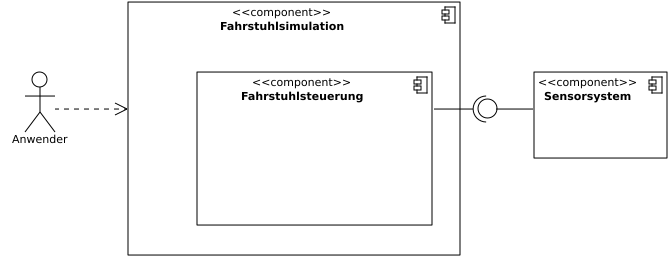
\includegraphics[width=\textwidth]{images/Kontextdiagramm.png}
	\caption{Kontextdiagramm der \gls{Fahrstuhlsimulation}}
	\label{fig:Kontextdiagramm}
\end{figure}

\vspace{0,5cm}

Im Kontext unseres Systems befinden sich der Anwender und ein Sensorsystem, dass über eine definierte Schnittstelle mit der \gls{Fahrstuhlsimulation} kommuniziert.

\newpage
\section{Satzschablonen}
Im Folgenden werden die Anforderungen an das Software-System mit Hilfe von Satzschablonen\footnote{Eine Satzschablone ist ein Bauplan für die syntaktische Struktur einer einzelnen Anforderung. Der Einsatz der Satzschablone unterstützt den Autor einer Anforderung darin, die syntaktische Eindeutigkeit der Anforderung zu erreichen. Dabei orientierten wir uns an den Strukturen von Chris Rupp. \url{http://goo.gl/Ony8c6}} dokumentiert. 

\paragraph{}
Deren Auflistung unterscheidet dabei zwischen selbstständigen Systemaktivitäten\footnote{Diese Aktionen werden von der \gls{Fahrstuhlsteuerung} selbstständig ausgeführt. Über verschiedene Schnittstellen interagieren Benutzer, Passagier und Sensoren mit dem System.} und Benutzerinteraktionen\footnote{Über Benutzerinteraktionen kann der Benutzer des Software-Systems mit der \gls{Fahrstuhlsteuerung} interagieren.}. Weiterhin wird eine Nummerierung vorgenommen, welche in allen Teilen der Software-und Projektdokumentation konsistent benutzt wird.

\paragraph{}
\textbf{Selbstständige Systemaktivitäten}
\begin{itemize}
	\item \textbf{ELV-001:} \newline
		Die \gls{Fahrstuhlsimulation} muss den Fahrstuhl nach oben fahren lassen.
	\item \textbf{ELV-002:} \newline
		Die \gls{Fahrstuhlsimulation} muss den Fahrstuhl nach unten fahren lassen.
	\item \textbf{ELV-003:} \newline
		Die \gls{Fahrstuhlsimulation} muss das Öffnen der Fahrstuhltür anzeigen.
	\item \textbf{ELV-004:} \newline
		Die \gls{Fahrstuhlsimulation} muss das Schließen der Fahrstuhltür anzeigen.
	\item \textbf{ELV-005:} \newline
		Die \gls{Fahrstuhlsimulation} sollte den aktuellen Zustand des Fahrstuhls anzeigen.
\end{itemize}

\newpage
\begin{itemize}
	\item \textbf{ELV-006:} \newline
		Die \gls{Fahrstuhlsimulation} sollte Zustandsübergänge des Fahrstuhls anzeigen.
	\item \textbf{ELV-007:} \newline
		Die \gls{Fahrstuhlsimulation} muss den Wechsel einer Etage anzeigen.
	\item \textbf{ELV-008:} \newline
		Die \gls{Fahrstuhlsimulation} sollte die Fahrstuhltür selbständig schließen, wenn 
		länger als 3 Sekunden keine Benutzerinteraktion durchgeführt wurde.
	\item \textbf{ELV-009:} \newline
		Die \gls{Fahrstuhlsimulation} muss eine \gls{Ueberlast} des Fahrstuhls durch zu 
		viele \gls{Passagier} anzeigen.
	\item \textbf{ELV-010:} \newline
		Die \gls{Fahrstuhlsimulation} muss im Falle einer Überlastsituation\footnote{Eine Überlastsituation tritt ein, sobald sich mehr als 8 Passagiere im Fahrstuhl befinden.} in den Zustand \gls{Ueberlast} wechseln. Ausgehend von diesem Zustand  ist es ausschließlich möglich in den vorherigen Zustand zu wechseln, sofern die Überlastsituation durch das Verlassen von Passagieren aufgehoben wurde.
\end{itemize}

\newpage
\paragraph{}
\textbf{Benutzerinteraktionen}
\begin{itemize}
	\item \textbf{ELV-011:}
		Die \gls{Fahrstuhlsimulation} muss dem Anwender die Möglichkeit bieten einen \gls{Fahrtwunsch}\footnote{Ein \gls{Fahrtwunsch} ist die Eingabe der Zieletage eines \gls{Passagier} über die innere Schaltfläche des Liftes.} für einen \gls{Passagier} einzugeben.
	\item \textbf{ELV-012:}
		Die \gls{Fahrstuhlsimulation} muss dem Anwender die Möglichkeit bieten einen \gls{Passagier} in den Fahrstuhl einsteigen zu lassen.
	\item \textbf{ELV-013:}
		Die \gls{Fahrstuhlsimulation} muss dem Anwender die Möglichkeit bieten einen \gls{Passagier} aus dem Fahrstuhl aussteigen zu lassen.
	\item \textbf{ELV-014:}
		Die \gls{Fahrstuhlsimulation} muss dem Anwender die Möglichkeit geben, einen \gls{Fahrstuhlruf}\footnote{Ein \textbf{\textit{Ruf}} wird durch das Betätigen eines Etagenknopfes abgesetzt.} in jedem Stockwerk absetzen zu können.
	\item \textbf{ELV-015:}
		Die \gls{Fahrstuhlsimulation} sollte dem Anwender die Möglichkeit bieten eine \gls{PrioFahrtwunsch} \footnote{Der Benutzer kann einen \textit{\gls{Monteur}} in den Lift einsteigen lassen, welcher die Möglichkeit besitzt einen \textit{\gls{PrioFahrtwunsch}} einzugeben.} auswählen zu lassen.
\end{itemize}

\newpage
\section{Anwendungsfälle - Benutzersicht}
In dieser Sicht gibt es einen \textit{\guillemotleft \ abstrakten \ \guillemotright} Anwendungsfall \textit{\textbf{\gls{Passagier}/\gls{Monteur} steuern}}. Dieser gliedert sich in die unabhängigen Anwendungsfälle:

\begin{itemize}
	\item \textit{\textbf{\gls{Passagier}-einsteigen}} (ELV-012)
	\item \textit{\textbf{\gls{Passagier}-aussteigen}} (ELV-013)
\end{itemize}

\begin{figure}[hbt]
	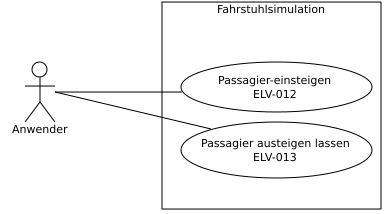
\includegraphics{images/anwenderAWF.png}
	\label{fig:anwenderAWF}
	\caption{Anwendungsfalldiagramm aus Sicht des Anwenders}
\end{figure}

Die Eingangs- und Ausgangsdaten sowie einige Bemerkungen zu den Anwendungsfällen sind in folgender Tabelle zusammengefasst.

 {
\vspace{1cm}
\hspace{-0,5cm}
\footnotesize
\begin{tabular}{|p{1,5cm}|p{2,5cm}|p{2,5cm}|p{2,5cm}|p{2cm}|}
	\hline
		\textbf{Funktion} &
		\textbf{Eingangsdaten} &
		\textbf{Ausgangsdaten} &
		\textbf{Bemerkungen} &
		\textbf{abstrakter AWD} \\
	\hline \hline
		\textit{Passagier \newline einsteigen} &
		Betätigung der entsprechenden Schaltfläche &
		Visuelle Bestätigung der Eingabe &
		Betreten mehr als 8 Personen den Lift kann eine Überlastsituation auftreten&
		\textbf{Passagier /\newline Monteur\newline steuern} \\
	\cline{1-4}
		\textit{Passagier \newline aussteigen} &
		Betätigung der entsprechenden Schaltfläche &
		Visuelle Bestätigung der Eingabe &
		&
		\\
	\hline
\end{tabular}
}

\section{Anwendungsfälle - Passagiersicht}
Aus dieser Perspektive ergeben sich drei voneinander unabhängige Anwendungsfälle:

\begin{itemize}
	\item \textit{\textbf{\gls{Fahrtwunsch} - Passagier}} (ELV-011)
	\item \textit{\textbf{\gls{Fahrstuhlruf} }} (ELV-014)
	\item \textit{\textbf{\gls{PrioFahrtwunsch}}} (ELV-015)
\end{itemize}


\begin{figure}[hbt]
	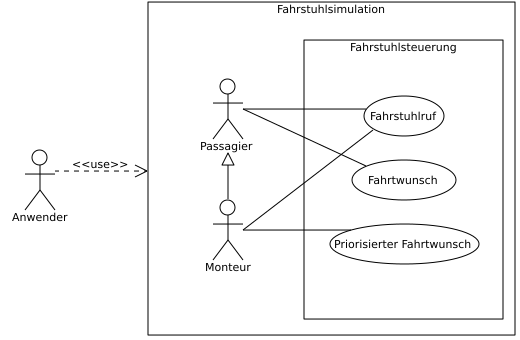
\includegraphics[width=\textwidth]{images/passagierAWF.png}
	\label{fig:passagierAWF}
	\caption{Anwendungsfalldiagramm aus Sicht des Passagieres}
\end{figure}
Beim \gls{Monteur} handelt es sich um eine Spezialisierte Form eines \gls{Passagier}s der die Möglichkeit besitzt einen \glslink{PrioFahrtwunsch}{priorisierten Fahrtwunsch} einzugeben. Die Eingangs-, Ausgangsdaten sowie Bemerkungen sind wiederum in folgender Tabelle zusammengefasst.

 {
\vspace{1cm}
\hspace{-0,5cm}
\footnotesize
\begin{tabular}{|p{2cm}|p{3cm}|p{3cm}|p{3cm}|}
	\hline
		\textbf{Funktion} &
		\textbf{Eingangsdaten} &
		\textbf{Ausgangsdaten} &
		\textbf{Bemerkungen} \\
	\hline \hline
		\textit{Fahrtwunsch \newline Passagier} &
		Etagenwahl (innen) &
		Leuchten der Wunschetage &
		Übergabe des Wunsches an Fahrstuhlsteuerung \\
	\hline
		\textit{Fahrstuhlruf} &
		Drücken eines der beiden Rufknöpfe (außen) &
		Leuchten der Ruftaste &
		Übergabe des Wunsches an Fahrstuhlsteuerung  \\
	\hline
		\textit{Fahrtwunsch \newline Monteur} &
		Drücken des Schlüsselsymbols und der Rufetage &
		Leuchten der des Schlüsselsymbols und der Wunschetage &
		Übergabe des Wunsches an Fahrstuhlsteuerung  \\
	\hline
\end{tabular}
}

\section{Qualitätsanforderungen}
Benutzerfreundlichkeit und die intuitive Bedienbarkeit des Software-Systems haben vor allem im Lehrbetrieb große Wichtigkeit. Aktivitäten des Systems sollten erst nach der Interaktion des Benutzers beginnen und nicht automatisch starten. So ist sicher gestellt, dass der Benutzer in jeder Situation ge\-nügend Zeit hat, um das vergangene und zukünftige Verhalten des Systems nachvollziehen und durchdenken zu können. 

\paragraph{}
Weiterhin wird sichergestellt, dass jede Interaktion des Benutzers mit dem System eine Rückmeldung an den Benutzer gibt. Hier werden vor allem Methoden der visuellen Rückmeldung Anwendung finden.

\section{Rahmenbedingungen}
In der Aufgabenstellung wurde die Bedingung formuliert, dass die \gls{Fahrstuhlsimulation} im Labor Z136b des HTW-Hauptgebäudes lauffähig sein muss. Damit ist die Mindestanforderung \textit{Lauffähigkeit auf Windows 7}. 

\paragraph{}
Darüber hinaus wurden in Absprache mit Frau Prof. Hauptmann verschiedene Webtechnologien wie bspw. \textsc{Javascript} als Basis für die Implementierung der \gls{Fahrstuhlsimulation} festgelegt. 
